% CVPR 2024 Paper Template; see https://github.com/cvpr-org/author-kit

\documentclass[10pt,twocolumn,letterpaper]{article}

%%%%%%%%% PAPER TYPE  - PLEASE UPDATE FOR FINAL VERSION
% \usepackage{cvpr}              % To produce the CAMERA-READY version
\usepackage[review]{cvpr}      % To produce the REVIEW version
% \usepackage[pagenumbers]{cvpr} % To force page numbers, e.g. for an arXiv version

% Import additional packages in the preamble file, before hyperref
%
% --- inline annotations
%
\usepackage{amsmath} 
\usepackage{amssymb} 
\usepackage[T1]{fontenc}
\usepackage{bm}
\nolinenumbers % 关闭行编号
\usepackage[dvipsnames]{xcolor}
\newcommand{\red}[1]{{\color{red}#1}}
\newcommand{\todo}[1]{{\color{red}#1}}
\newcommand{\TODO}[1]{\textbf{\color{red}[TODO: #1]}}
% --- disable by uncommenting  
% \renewcommand{\TODO}[1]{}
% \renewcommand{\todo}[1]{#1}



% It is strongly recommended to use hyperref, especially for the review version.
% hyperref with option pagebackref eases the reviewers' job.
% Please disable hyperref *only* if you encounter grave issues, 
% e.g. with the file validation for the camera-ready version.
%
% If you comment hyperref and then uncomment it, you should delete *.aux before re-running LaTeX.
% (Or just hit 'q' on the first LaTeX run, let it finish, and you should be clear).
\definecolor{cvprblue}{rgb}{0.21,0.49,0.74}
\usepackage[pagebackref,breaklinks,colorlinks,citecolor=cvprblue]{hyperref}

%%%%%%%%% PAPER ID  - PLEASE UPDATE
\def\paperID{*****} % *** Enter the Paper ID here
\def\confName{CVPR}
\def\confYear{2024}

%%%%%%%%% TITLE - PLEASE UPDATE
%\title{\LaTeX\ Author Guidelines for \confName~Proceedings}
\title{A Brain-Inspired Perception and Decision Driving Model Based on Neural Pathway Anatomical Alignment}
%%%%%%%%% AUTHORS - PLEASE UPDATE
\author{First Author\\
Institution1\\
Institution1 address\\
{\tt\small firstauthor@i1.org}
% For a paper whose authors are all at the same institution,\part{\part{title}}
% omit the following lines up until the closing ``}''.
% Additional authors and addresses can be added with ``\and'',
% just like the second author.
% To save space, use either the email address or home page, not both
\and
Second Author\\
Institution2\\\usepackage{bm}
First line of institution2 address\\
{\tt\small secondauthor@i2.org}
}
\begin{document}
\maketitle
\begin{abstract}
In the realm of autonomous driving, conventional approaches to vehicle perception and decision-making primarily rely on sensor input and rule-based algorithms. However, these methodologies often suffer from lack of interpretability and robustness, particularly in intricate traffic scenarios. To tackle this challenge, we propose a novel BID(Brain-Inspired Driving) framework. Diverging from traditional methods, our approach harnesses brain-inspired perception technology to achieve more efficient and robust environmental perception. Additionally, it employs brain-inspired decision-making techniques to facilitate intelligent decision-making. The experimental results show that the performance has been significantly improved across various autonomous driving tasks and achieved the end-to-end autopilot successfully. This contribution not only advances interpretability and robustness but also offers fancy insights and methodologies for further advancing autonomous driving technology.
\end{abstract}
    
\section{Introduction}
\label{sec:intro}
\hspace{1pc}Autonomous driving \cite{urmson2008autonomous} is an advanced technology that intelligent vehicles perceive road environments through onboard sensor systems, autonomously plan driving routes, and control vehicles to reach predetermined destinations. Its technical system generally includes three major parts: environmental perception, decision planning, and vehicle control \cite{amini2020learning, montemerlo2008junior}, involving multiple research fields such as computer science, mathematics, mechanical engineering, control science, and psychology \cite{chen2015deepdriving}.

However, the current autonomous driving systems still suffer from insufficient interpretability due to the existence of "black box" nature of deep learning models \cite{7979332}, greatly limiting the credibility and widespread application of various perception and decision-making methods in practical engineering. Even though the use of generative adversarial networks (GANs) \cite{zugner2020adversarial} to generate explanatory data related to decision-making has been attempted, the quality of such data is often substandard, and the training process is quite challenging. Furthermore, modern urban traffic conditions are characterized by high dynamics and strong uncertainty. When the environment is complex, the autonomous driving system may experience performance degradation. Therefore, to overcome the limitations of existing methods, there is a need to design more interpretable and robust autonomous driving systems, thereby ensuring the safety of vehicle operation.
\begin{figure}[t]
	\centering
	%\fbox{\rule{0pt}{2in} \rule{0.9\linewidth}{0pt}}
	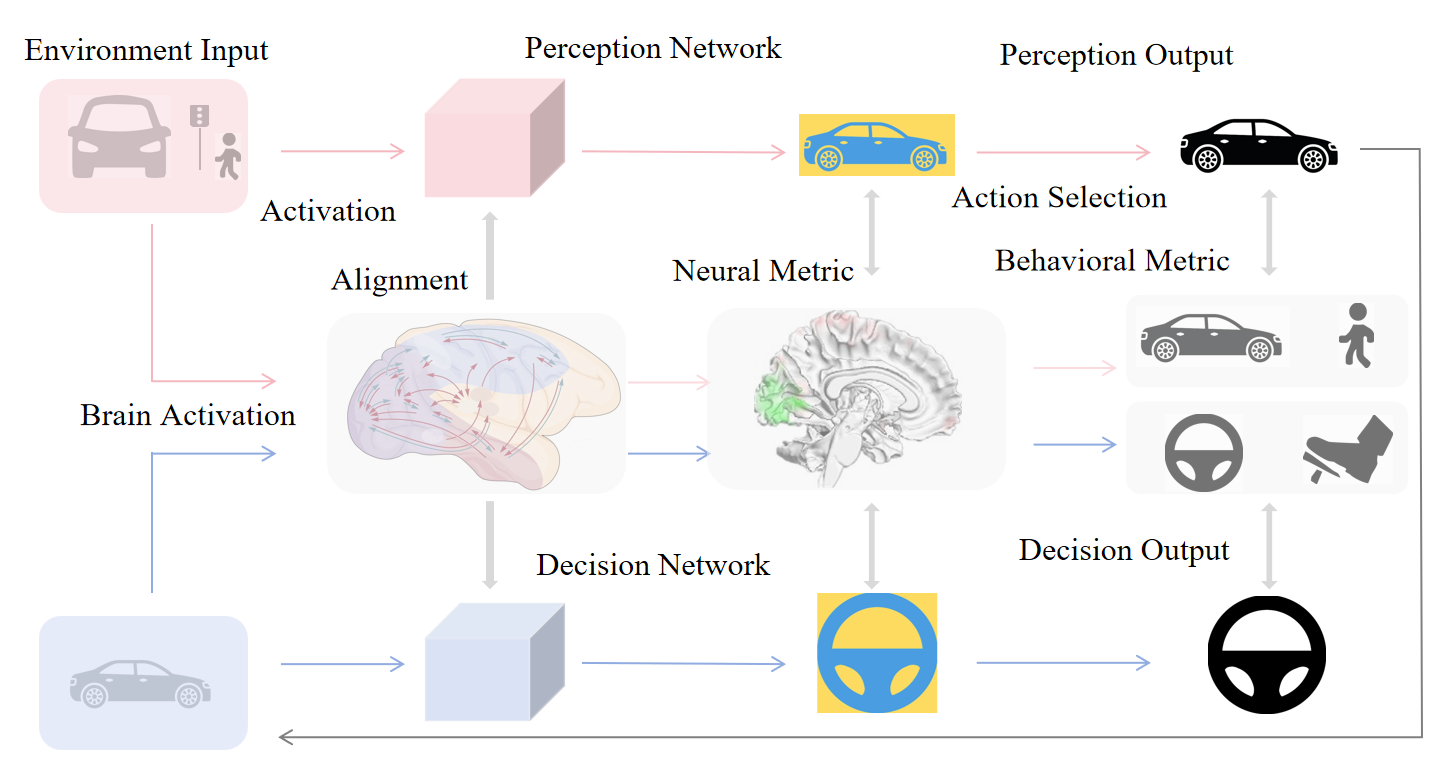
\includegraphics[width=0.8\linewidth]{brain_inspired.png}
	
	\caption{Brain-inspired Perception and Decision Network}
	\label{fig:fig1}
\end{figure}

In this paper, we propose a novel BID framework based on brain-inspired perception and decision-making. Unlike previous methods, our reinforcement learning expert does not rely on manually formulated rules and demonstrates strong interpretability and robustness. Our work involves constructing a brain-inspired perception network for extracting environmental features of the target vehicle and a brain-inspired decision-making network for generating driving decisions for the target vehicle, in order to train the reinforcement learning expert \cite{kahn2021land}. Its structure is as shown in Fig. \ref{fig:fig1}. Specifically, the brain-inspired perception network consists of a visual perception module \cite{al2018brain}, a motion perception module, and a multimodal perception module \cite{yu2023brain}. The brain-inspired decision-making network comprises a decision generation module \cite{schirner2023learning} and a decision evaluation module. Driving decisions encompass multiple driving actions of the target vehicle, and the BID agent directly imitates expert behavior. Overall, our main contribution lies in proposing a novel brain-inspired perception model and a brain-inspired decision-making model for autonomous driving, aiming to achieve a more robust and interpretable autonomous driving system.
\section{Related Work}
\subsection{Brain-Inspired Perception}
\hspace{1pc}The human visual cortex possesses remarkable environmental perception capabilities, serving as a crucial component of the central nervous system and responsible for transforming visual signals into comprehensible information \cite{9134376}. Traditional visual encoding models are limited by the use of either handcrafted or deep learning features merely, despite their individual advantages. To integrate the two, Cui et al. \cite{8574054} proposed the GaborNet-VE model, which combines Gabor features with deep learning to form an efficient visual encoding framework. However, this model requires significant parameter adjustments across different tasks, and the interpretability of its deep learning component remains inadequate. In contrast, our proposed BID  model demonstrates outstanding performance in revealing decision-making mechanisms and exhibiting strong generalization capabilities.
\subsection{Brain-Inspired Decision}
\hspace{1pc}In practical environments, agents often need to handle continuous state spaces, while traditional reinforcement learning models, such as Q-learning and Actor-Critic algorithms, are more suitable for discrete states. To address this issue, Zhao et al. \cite{zhao2018brain} proposed the prefrontal cortex-basal ganglia (PFC-BG) algorithm, which subdivides continuous states and introduces continuous reward functions to capture temporal reward information. However, the design of continuous reward functions remains a challenge. In non-Gaussian and nonlinear environments (NGNLE), traditional methods struggle to cope with their nonlinear and non-Gaussian characteristics. Inspired by human brain decision-making, Naghshvarianjahromi et al. \cite{8932505} designed an autonomous computation layer based on a cognitive dynamic system (CDS), providing agents in NGNLE with stronger decision-making capabilities. Although these methods attempt to mimic the decision-making process of the human brain, structural differences lead to a lack of transparency in their processes. Therefore, it is crucial to construct network models that align with the anatomical structure of human brain.
\section{Method}
\begin{figure*}[t]
	\centering
	%\fbox{\rule{0pt}{2in} \rule{0.9\linewidth}{0pt}}
	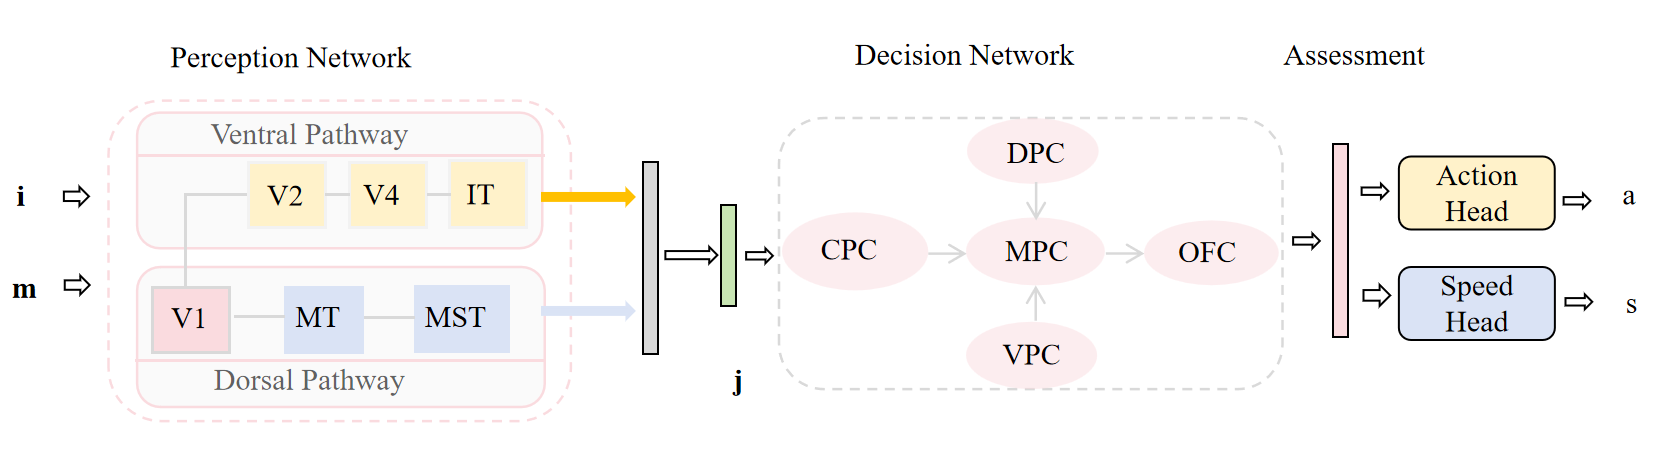
\includegraphics[width=\linewidth]{net.png}
	
	\caption{Network architecture of Roach and the BID agent.
	}
	\label{fig:fig2}
\end{figure*}
\subsection{Neural Aligned Roach}
\hspace{1pc}Drawing inspiration from the brain's exceptional mechanisms in perception and decision-making, we have seamlessly integrated the intricate methods of information processing by brain neurons into an autonomous driving system, aiming to significantly enhance the system's interpretability and robustness. As depicted in Fig. \ref{fig:fig2}, our brain-inspired perception network initially captures precise input data from the surrounding environment, encompassing crucial traffic elements such as roads, vehicles, pedestrians, and traffic signals. Subsequently, this data undergoes meticulous processing through a series of deep convolutional neural networks and recurrent networks, along with the utilization of deep neural network activation functions. This processing mimics the handling of external information by various pathways in the brain's visual cortex. Initially, the primary visual cortex (V1) performs initial processing of visual information, extracting salient features. These features are then relayed to the dorsal visual pathway, where the MT/MST (Middle Temporal and Middle Superior Temporal Areas) encode motion features, specializing in the processing of information related to spatial location and movement. Concurrently, the ventral pathway receives these features, and the IT (Inferior Temporal Cortex) encodes target category information, facilitating object recognition. After this series of processing, our network is able to effectively extract and output multi-dimensional features of the current environment, including the appearance features of objects, motion trajectory features, and the fusion of multi-modal information.

These features are then efficiently transmitted to a brain-inspired decision-making network, undergoing further processing through convolutional and recurrent networks, as well as optimization via deep neural network activation functions. This simulates the processing of sensory outcomes by various regions of the prefrontal cortex in the brain. Among them, the OFC (Orbitofrontal Cortex) plays a vital role in setting future action goals, assisting us in clarifying and locking onto the desired objectives. The MPC ( Medial Prefrontal Cortex) plays a crucial role in making choices based on prior behavioral outcomes, ensuring that our behavior is optimized based on experience. The DPC (Dorsal Prefrontal Cortex) excels at generating goals based on sequences, temporal and spatial environments, providing clear directions and guidance for our actions. The VPC (Ventral Prefrontal Cortex) generates goals based on visual and auditory cues, enabling us to respond quickly and adapt to changes in the external environment.  Meanwhile, the CPC (Caudal Prefrontal Cortex) plays an indispensable role in searching, identifying, or locating specific targets, ensuring that we can accurately locate and focus on the targets.  These regions collaborate and participate in decision-making, generating a highly integrated latent feature vector that precisely encapsulates the critical information required for decision-making. Finally, this latent feature vector is mapped through a carefully designed hidden layer, outputting precise and reliable decision-making information such as driving actions, value function estimates, and speed control.

\textbf{\textsf{Reward Function.}} The BID network aims to mimic the superior information processing capabilities of the human brain by meticulously comparing brain activation patterns with network activation patterns. It iteratively updates its network parameters to align network decisions more closely with the actual decision-making mechanisms of the human brain, thereby enhancing the performance and accuracy of the network. The specific methodology for updating the network is outlined as follows:
\begin{align}
	\theta_{k+1} & = \arg \max _{\theta} \underset{\tau \sim \pi_{\theta_{k}}}{\mathrm{E}}\left[\mathcal{L}_{\mathrm{ppo}}+\mathcal{L}_{\text {pre }}+\lambda_{\text {e }} \cdot \mathcal{L}_{\text {exp }}\right]
\end{align}

Simulating the approach the brain acquires rewards, aiming to maximize reward-seeking behavior. We train the decision network using Proximal Policy Optimization (PPO) \cite{schulman2017proximal} with clipping. $\mathcal{L}_{\text {ppo }}$ serves as the dopamine reward signal. It is understood that when the brain predicts an upcoming reward, the dopamine system becomes active, generating a reward signal. This signal can be seen as feedback from the brain regarding specific behaviors or situations, informing the brain whether the behavior or situation is positive or worth pursuing. $\mathcal{L}_{\text {pre }}$ represents the prediction error of brain reward. This error arises when there is a deviation between the actual reward and the expected reward. In this context, the reward prediction error functions as a penalty term. Specifically, if the actual reward ($a_{r}$) falls below the expected reward ($p_{r}$), the reward prediction error is negative.Additionally, $\mathcal{L}_{\text {exp }}$ encapsulates the exploration of new actions or strategies during the learning process to obtain more rewards, with $\lambda$ serving as their weight parameter.

Considering both the certainty of the policy (via the entropy regularization term) and the accuracy of reward prediction (via the reward prediction error term), this guides the model to learn more accurate reward predictions, thereby enhancing its performance in reinforcement learning tasks. Specifically, The constant (C) serves to adjust the numerical range or optimization scale of the entropy.
\begin{align}
	\mathcal{L}_{\text{pre}} & = -\lambda_{\text {p }} \cdot [\mathrm{H}\left(\pi_{\theta}\left(\cdot \mid \mathbf{i}_{\mathrm{NR}}, \mathbf{m}_{\mathrm{NR}}\right)\right) - (a_{r} - p_{r})^{2}]
\end{align}
\begin{align}
	\mathrm{H}\left(\pi_{\theta}\right) & = -\mathrm{KL}\left(\pi_{\theta} \| \mathcal{U}(-1,1)\right)+C
\end{align}

Regularizing the whole trajectory to better utilize previous experience and improve the efficiency and stability of learning.
\begin{align}
    \mathcal{L}_{\text {exp }}=\sum_{k=1}^{T} f(k) \cdot \mathrm{KL}\left(\pi_{\theta}\left(\cdot \mid \mathbf{i}_{\mathrm{NR}, k}, \mathbf{m}_{\mathrm{NR}, k}\right) \| p_{z}\right)
\end{align}

\textbf{\textsf{Training.}} The vehicle solely utilizes a single camera sensor to capture raw data of its surrounding environment. At the input stage, it receives a Bird's Eye View (BEV) semantic segmentation image, denoted as $\mathbf{i}_{\mathrm{NR}}$, along with a measurement vector, $\mathbf{m}_{\mathrm{NR}}$, from its own roach system. After acquiring these input data, the BID network is activated to simulate the brain's visual processing. When predicting or receiving rewards, simulated dopamine neurons are activated, releasing dopamine to strengthen memories and behaviors associated with the rewards, increasing the likelihood of repeating these behaviors. During the learning process, there is often a mismatch between expected and actual rewards. When actual rewards exceed expectations, a positive prediction error occurs, further promoting the release of dopamine and thus enhancing the associated behaviors. Through ongoing interaction with the environment, the brain-inspired network adapts behavioral policies by modifying parameters through backpropagation, striving to maximize future rewards.

Multiple driving actions are generated and evaluated separately to assign them respective scores. The driving action with the highest score is then selected to control the movement of the target vehicle.
%\begin{align}
%	S & = r_{1} \mu+r_{2} \lambda
%\end{align}
\subsection{Brain-Expert Mimetic Entity}
\hspace{1pc}\textbf{\textsf{Agent.}} The BID agent utilizes imitation learning to predict driving behavior based on the current state, supervised by extensive data generated by the reinforcement learning expert. The structure of the agent is illustrated in Fig. \ref{fig:fig2}.

\textbf{\textsf{Loss Function.}} In the decision-making stage, for each command, a branch is constructed. All branches share the same architecture, with each branch containing an action head for predicting the continuous action $\mathbf{a}$ and a velocity head for predicting the current vehicle speed $\mathbf{s}$. And $\mathbf{\hat{a}}$ represents the expert's action,$\mathbf{\hat{s}}$ is the measured speed, and $\mathbf{a}$ and $\mathbf{s}$ are the actions and speeds predicted by the agent, respectively. 
\begin{align}
   \mathcal{L} = \|\hat{\mathbf{a}}-\mathbf{a}\|_{1}^{2} + \lambda_{\mathrm{S}} \cdot (\hat{s}-s)^{2} + \lambda_{\mathrm{F}} \cdot \left\| \mathbf{j}_{\mathrm{NR}}-\mathbf{j}_{\mathrm{BID}} \right\|_{2}^{2}
\end{align}

Furthermore, the outputs of the brain-inspired perception network and the brain-inspired decision network are concatenated to produce a latent feature that encapsulates essential information for driving. This latent feature is then processed through a hidden layer to map it to driving actions. Hence, it also includes a feature loss.
\subsection{Similarity Measure}
\hspace{1pc}\textbf{\textsf{Collecting Brain Activation Signals.}} To align the network, we collect the brain's responses to multi-channel grayscale images. Initially, EEG sensors are placed at appropriate locations and connected to data acquisition equipment. Subsequently, neuroimaging software is utilized to preprocess cortical activation data. Then, the brain data is aligned with standard data to ensure consistency, followed by noise removal and data smoothing. Ultimately, we obtain activation signals from visual brain regions that vary over time as participants view different images. These signals are further amplified through deconvolution processing to reveal the brain's activation patterns.

\textbf{\textsf{Network Alignment.}} To achieve a closer alignment with human brain functions, the network parameters are continuously optimized, thereby significantly enhancing the bionic performance and simulation accuracy of the network.

\textbf{\textsf{Similarity Assessment.}} After parameter tuning, the BID network is capable of simulating the mechanisms of the human brain in environmental recognition and decision-making. Following each optimization, we accurately calculate the similarity between the BID and the human brain. The degree of congruency between the brain-inspired network and the human brain is quantified by computing the average of activation similarity and decision similarity through the specified formula. Notably, $S_{X_{p}}$ and $S_{X_{d}}$ denote the standard deviations of the model's activation sample points and decision sample points, respectively, whereas $S_{Y}$ represents the corresponding data values of the human brain.
\begin{align}
	r & = \frac{1}{2}\left(\frac{Cov_{X_{p},Y_{p}}}{\sqrt{S_{X_{p}} S_{Y_{p}}}}+\frac{Cov_{X_{d},Y_{d}}}{\sqrt{S_{X_{d}} S_{Y_{d}}}}\right)
\end{align}
%\begin{align}
%	r & = \frac{1}{2}\left(\frac{\sum_{i = 1}^{n}\left(X_{p_{i}}-\bar{X_{p}}\right)\left(Y_{p_{i}}-\bar{Y_{p}}\right)}{\sqrt{\sum_{i = 1}^{n}\left(X_{p_{i}}-\bar{X_{p}}\right)^{2}} \sqrt{\sum_{i = 1}^{n}\left(Y_{p_{i}}-\bar{Y_{p}}\right)^{2}}} \right. \nonumber \\
%	& \qquad \left. + \frac{\sum_{i = 1}^{n}\left(X_{d_{i}}-\bar{X_{d}}\right)\left(Y_{d_{i}}-\bar{Y_{d}}\right)}{\sqrt{\sum_{i = 1}^{n}\left(X_{d_{i}}-\bar{X_{d}}\right)^{2}} \sqrt{\sum_{i = 1}^{n}\left(Y_{d_{i}}-\bar{Y_{d}}\right)^{2}}} \right)
%\end{align}
\section{Experiment}
\begin{figure}[t]
	\centering
	%\fbox{\rule{0pt}{2in} \rule{0.9\linewidth}{0pt}}
	\includegraphics[width=0.8\linewidth]{experiment.png}
	
	\caption{Assessing the Similarity Between Network Activation and Brain Activation.}
	\label{fig:fig3}
\end{figure}
\label{sec:experiment}
\hspace{1pc}\textbf{\textsf{Implementation Details.}} During the experiment, we randomly selected start and target positions, and computed the route using A* algorithm. Subsequently, we executed $\pi_{\theta_{k}}$ in the CARLA \cite{Dosovitskiy17} environment to gather trajectory data and synchronized brain activation record. We employed a specific reward scheme and imposed additional penalties for large steering changes to prevent oscillatory maneuvers. After training the network, we compared the similarity between the network activations and those observed in the human brain. As depicted in Fig. \ref{fig:fig3}, we contrasted the similarity between the test participant and the brain-inspired network in processing the same event.

\textbf{\textsf{Performance of BID.}} The performance of the BID agent is constrained by the performance of the expert it is imitating. When the expert performs poorly, the agent that mimics the expert will also exhibit poor performance. The BID model is designed in strict accordance with the human brain's visual information processing process, both structurally and functionally. When optimized, the model's output results are very close to those of the human brain in terms of evaluating the similarity in activation. 
\section{Conclusion}
\label{sec:conclusion}
\hspace{1pc}This paper delves into the application of the BID model in brain-inspired autonomous driving. The model aims to replicate how pathways in the brain's visual and decision-making regions process information, aiming to boost the interpretability and robustness of autonomous driving systems by mimicking biological neural mechanisms. Apart from visual cue perception, the BID model focuses on optimizing decision-making strategies by simulating the release of dopamine to achieve higher reward signals. This dopamine-mimicking approach helps autonomous driving systems balance risks and rewards intelligently in complex traffic, ultimately enhancing safety and robustness.
\newpage
{
    \small
    \bibliographystyle{ieeenat_fullname}
    \bibliography{main}
}

% WARNING: do not forget to delete the supplementary pages from your submission 
% \clearpage
\setcounter{page}{1}
\maketitlesupplementary


\section{Rationale}
\label{sec:rationale}
% 
Having the supplementary compiled together with the main paper means that:
% 
\begin{itemize}
\item The supplementary can back-reference sections of the main paper, for example, we can refer to \cref{sec:intro};
\item The main paper can forward reference sub-sections within the supplementary explicitly (e.g. referring to a particular experiment); 
\item When submitted to arXiv, the supplementary will already included at the end of the paper.
\end{itemize}
% 
To split the supplementary pages from the main paper, you can use \href{https://support.apple.com/en-ca/guide/preview/prvw11793/mac#:~:text=Delete%20a%20page%20from%20a,or%20choose%20Edit%20%3E%20Delete).}{Preview (on macOS)}, \href{https://www.adobe.com/acrobat/how-to/delete-pages-from-pdf.html#:~:text=Choose%20%E2%80%9CTools%E2%80%9D%20%3E%20%E2%80%9COrganize,or%20pages%20from%20the%20file.}{Adobe Acrobat} (on all OSs), as well as \href{https://superuser.com/questions/517986/is-it-possible-to-delete-some-pages-of-a-pdf-document}{command line tools}.

\end{document}
